% move all configuration stuff into one file so we can focus on the content
\documentclass[aspectratio=169,hyperref={pdfpagelabels=false,colorlinks=true,linkcolor=white,urlcolor=blue},t]{beamer}

%%%%%%%%%%%%%%%%%%%%%%%%%%%%%%%%%%%%%%%%%%%%%%%%%%%%%%%%%%%%%%%%%%%%%%%%%%%%%%%%%%
%%%%%%%%%%%%%%%%%%%%%%%%%%%%%%%%%%%%%%%%%%%%%%%%%%%%%%%%%%%%%%%%%%%%%%%%%%%%%%%%%%
% packages
\usepackage{pict2e}
\usepackage{epic}
\usepackage{amsmath,amsfonts,amssymb}
\usepackage{units}
\usepackage{fancybox}
\usepackage[absolute,overlay]{textpos} 
\usepackage{media9} % avi2flv: "C:\Program Files\ffmpeg\bin\ffmpeg.exe" -i TuneFreqFilterbank.avi -b 600k -s 441x324 -r 15 -acodec copy TuneFreqFilterbank.flv
\usepackage{animate}
\usepackage{gensymb}
\usepackage{multirow}
\usepackage{silence}
\usepackage[backend=bibtex,style=ieee]{biblatex}
\AtEveryCitekey{\iffootnote{\tiny}{}}
\addbibresource{references}

%%%%%%%%%%%%%%%%%%%%%%%%%%%%%%%%%%%%%%%%%%%%%%%%%%%%%%%%%%%%%%%%%%%%%%%%%%%%%%%%%%
%%%%%%%%%%%%%%%%%%%%%%%%%%%%%%%%%%%%%%%%%%%%%%%%%%%%%%%%%%%%%%%%%%%%%%%%%%%%%%%%%%
% relative paths
\graphicspath{{graph/}}


%%%%%%%%%%%%%%%%%%%%%%%%%%%%%%%%%%%%%%%%%%%%%%%%%%%%%%%%%%%%%%%%%%%%%%%%%%%%%%%%%%
%%%%%%%%%%%%%%%%%%%%%%%%%%%%%%%%%%%%%%%%%%%%%%%%%%%%%%%%%%%%%%%%%%%%%%%%%%%%%%%%%%
% units
\setlength{\unitlength}{1mm}

%%%%%%%%%%%%%%%%%%%%%%%%%%%%%%%%%%%%%%%%%%%%%%%%%%%%%%%%%%%%%%%%%%%%%%%%%%%%%%%%%%
%%%%%%%%%%%%%%%%%%%%%%%%%%%%%%%%%%%%%%%%%%%%%%%%%%%%%%%%%%%%%%%%%%%%%%%%%%%%%%%%%%
% theme & layout
\usetheme{Frankfurt}
\beamertemplatenavigationsymbolsempty
%\setbeamertemplate{frametitle}[smoothbars theme]
\setbeamertemplate{frametitle}
{
    \begin{beamercolorbox}[ht=1.8em,wd=\paperwidth]{frametitle}
        \vspace{-.1em}%
        \hspace{.2em}{\strut\insertframetitle\strut}
        
        \hspace{.2em}\small\strut\insertframesubtitle\strut
        %\hfill
        %
\includegraphics[height=.8cm,keepaspectratio]{CenterMusicTechnology-solid-2lines-white-CoAtag}
        
    \end{beamercolorbox}
    \begin{textblock*}{100mm}(11.6cm,.7cm)
        \includegraphics[height=.8cm,keepaspectratio]{logo_GTCMT_black}
    \end{textblock*}
}

% set this to ensure bulletpoints without subsections
\usepackage{remreset}
\makeatletter
\@removefromreset{subsection}{section}
\makeatother
\setcounter{subsection}{1}

%---------------------------------------------------------------------------------
% appearance
\setbeamercolor{structure}{fg=gtgold}
\setbeamercovered{transparent} %invisible
\setbeamercolor{bibliography entry author}{fg=black}
\setbeamercolor*{bibliography entry title}{fg=black}
\setbeamercolor*{bibliography entry note}{fg=black}

%\usepackage{pgfpages}
%\setbeameroption{show notes}
%\setbeameroption{show notes on second screen=right}
%---------------------------------------------------------------------------------
% fontsize
\let\Tiny=\tiny

%%%%%%%%%%%%%%%%%%%%%%%%%%%%%%%%%%%%%%%%%%%%%%%%%%%%%%%%%%%%%%%%%%%%%%%%%%%%%%%%%%
%%%%%%%%%%%%%%%%%%%%%%%%%%%%%%%%%%%%%%%%%%%%%%%%%%%%%%%%%%%%%%%%%%%%%%%%%%%%%%%%%%
% warnings
\pdfsuppresswarningpagegroup=1
\WarningFilter{biblatex}{Patching footnotes failed}
\WarningFilter{latexfont}{Font shape}
\WarningFilter{latexfont}{Some font shapes}
\WarningFilter{gensymb}{Not defining}



\subtitle{Part 6.2: Monophonic Fundamental Frequency Detection}

%%%%%%%%%%%%%%%%%%%%%%%%%%%%%%%%%%%%%%%%%%%%%%%%%%%%%%%%%%%%%%%%%%%%%%%%%%%%
\begin{document}
    % generate title page
	

\begin{frame}
    \titlepage
    %\vspace{-5mm}
    \begin{flushright}
        \href{http://www.gtcmt.gatech.edu}{\includegraphics[height=.8cm,keepaspectratio]{logo_GTCMT_black}}
    \end{flushright}
\end{frame}


    \section[overview]{lecture overview}
        \begin{frame}{fundamental frequency detection}{overview}
            \begin{itemize}
                \item   \textbf{text book}  
                    \begin{itemize}
                        \item   \href{http://ieeexplore.ieee.org/xpl/articleDetails.jsp?tp=&arnumber=6331122&}{\underline{\textit{Chapter 5: Tonal Analysis} (pp.~94--111)}}
                    \end{itemize}
                \bigskip
                \item<2->   \textbf{lecture content}
                    \begin{itemize}
                        \item<2->   pitch tracking (monophonic)
                            \begin{itemize}
                                \item   time domain
                                \item   frequency domain
                            \end{itemize}
                    \end{itemize}
            \end{itemize}
        \end{frame}

    \section[intro]{introduction}
	\begin{frame}{fundamental frequency}{introduction}
        \begin{block}{\textbf{remember}}
            Fourier series: every (quasi-)periodic sound is a combination of sinusoidals with integer frequency ratios
        \end{block}
        \begin{eqnarray*}
            x(t) 	&\approx& x(t+T_0)\nonumber\\
            x(t) &\approx& \sum\limits_{k=-\infty}^{\infty} a(k) \e^{\jom_0kt}\nonumber
        \end{eqnarray*}
        
		\begin{itemize}
			\item<2->[]	$f_0$: musically, perceptually most ``relevant'' frequency
		\end{itemize}
        \only<2->{
        \begin{figure}[t]
            \centering
            
\includegraphics[scale=.7]{pitch_harmonics}
        \end{figure}
        }
	\end{frame}
	
	\begin{frame}{fundamental frequency detection}{monophonic --- pre-processing}
		examples for pre-processing steps
		\begin{itemize}
			\item	\textbf{downmixing}:\\ identical fundamental frequency in all channels
			\pause
			\item	\textbf{low-pass filter}:\\ cut off high partials
			\pause
			\item	\textbf{high-pass filter}:\\ remove DC and unnecessary bass frequencies
			\pause
			\item	(\textbf{pre-whitening}:)\\ remove spectral envelope to receive time domain pulse train
			\item	\ldots
		\end{itemize}
	\end{frame}
    
    \section[time domain]{monophonic pitch tracking}

	
	\begin{frame}{fundamental frequency detection}{monophonic --- zero crossing rate}
		\begin{itemize}
			\item	\textbf{number of zero crossings per block}
				\begin{equation*}
					T_0(n) = \frac{2\cdot \big(i_{\mathrm{e}}(n)-i_{\mathrm{s}}(n)\big)}{f_{\mathrm{S}}\cdot\sum\limits_{i=i_{\mathrm{s}}(n)}^{i_{\mathrm{e}}(n)}{\left|\sign \left[x(i)\right]-\sign \left[x(i-1)\right]\right|}} 
				\end{equation*}
			\pause
			\item	\textbf{average period length}
				\begin{equation*}
					T_0(n) = \frac{2}{\mathcal{Z}-1}\sum\limits_{z=0}^{\mathcal{Z}-2}{\Delta t_\mathrm{ZC}(z)}.
				\end{equation*}
			\pause
			\item	\textbf{variants}:
				\pause
				\begin{itemize}
					\item	create histogram with distances and choose maximum
					\pause
					\item	use not (only) ZC but distance between local extrema
				\end{itemize}
		\end{itemize}
	\end{frame}
	
	\begin{frame}{fundamental frequency detection}{monophonic --- auto correlation function}
		\begin{equation*}
			r_{xx}(\eta,n) = \sum\limits_{i=i_{\mathrm{s}}(n)}^{i_{\mathrm{e}}(n)-\eta}{x(i)\cdot x(i+\eta)}
		\end{equation*}
		\pause
		$\Rightarrow$ \textbf{detect maximum location}
		
		\pause
		variants:
		\begin{itemize}
			\item	center clipping
					\begin{figure}
					  	\centering
						\begin{footnotesize}
	\begin{picture}(80,37)

	%%%%%%%%%%%%%%%%%%%%%%%%%%%
	% normal center clipping	
	\put(0, 21)
	{\vector(1,0){32}}
	\put(16, 5)
	{\vector(0,1){32}}
	
	\put(30, 23)
	{\text{{\shortstack[c]{$x$}}}}
	
	\put(8, 35)
	{\text{{\shortstack[c]{$\chi(x)$}}}}
	
	\put(2, 18)
	{\text{{\footnotesize{\shortstack[c]{$-c_\mathrm{L}$}}}}}
	
	\put(22, 18)
	{\text{{\footnotesize{\shortstack[c]{$+c_\mathrm{L}$}}}}}


	%%%%%%%%%%%%%%%%%%%%%%%%%%%
	% 3-level center clipping	
	\put(48, 21)
	{\vector(1,0){32}}
	\put(64, 5)
	{\vector(0,1){32}}

	\put(63.5, 13)
	{\line(1,0){1}}
	\put(63.5, 29)
	{\line(1,0){1}}
	
	\put(78, 23)
	{\text{{\shortstack[c]{$x$}}}}
	
	\put(56, 35)
	{\text{{\shortstack[c]{$\chi'(x)$}}}}
	
	\put(50, 18)
	{\text{{\footnotesize{\shortstack[c]{$-c_\mathrm{L}$}}}}}
	
	\put(70, 18)
	{\text{{\footnotesize{\shortstack[c]{$+c_\mathrm{L}$}}}}}
	
	\put(65, 13)
	{\text{{\footnotesize{\shortstack[c]{$-1$}}}}}
	
	\put(65, 29)
	{\text{{\footnotesize{\shortstack[c]{$+1$}}}}}
	
	
	% transfer functions

	\linethickness{0.5mm}	
	
	\put(8, 21)
	{\line(0,-1){8}}
	\put(24, 21)
	{\line(0,1){8}}
	\put(8, 13)
	{\line(-1,-1){8}}
	\put(24, 29)
	{\line(1,1){8}}
	\put(8, 21)
	{\line(1,0){16}}
	
	
	\put(56, 21)
	{\line(0,-1){8}}
	\put(72, 21)
	{\line(0,1){8}}
	\put(56, 13)
	{\line(-1,0){8}}
	\put(72, 29)
	{\line(1,0){8}}
	\put(56, 21)
	{\line(1,0){16}}

	\end{picture}
\end{footnotesize}

					  	\label{fig:centerclipping}
					\end{figure}
			\pause
			\item	pre-whitening: LP, spectral envelope estimation															
		\end{itemize}
	\end{frame}
	
	\begin{frame}{fundamental frequency detection}{monophonic --- average magnitude difference function}
		\begin{equation*}
			\mathrm{AMDF}_{xx}(\eta,n) = \frac{1}{i_{\mathrm{e}}(n)-i_{\mathrm{s}}(n)+1}\sum\limits_{i=i_{\mathrm{s}}(n)}^{i_{\mathrm{e}}(n)-\eta}{|x(i)- x(i+\eta)|} 
		\end{equation*}
		\pause
		$\Rightarrow$ \textbf{detect minimum location}
		
		\pause
		\vspace{3mm}
		variants:
		\begin{itemize}
			\item	AMDF-weighted ACF
				\begin{equation*}
					r_{xx}'(\eta,n) = \frac{r_{xx}(\eta,n)}{\mathrm{AMDF}_{xx}(\eta,n) + 1} 
				\end{equation*}
		\end{itemize}
	\end{frame}
	
    \section[frequency domain]{monophonic pitch tracking}
	\begin{frame}{fundamental frequency detection}{monophonic --- harmonic product spectrum 1/2}
        \vspace{-15mm}
        \begin{columns}
            \column{0.5\textwidth}
                \vspace{4mm}
                \begin{equation*}\label{eq:hps}
                    X_{\mathrm{HPS}}(k,n) = \prod\limits_{j=1}^{\mathcal{O}}{|X(j\cdot k,n)|^2}
                \end{equation*}
                
                first published in the 1960s by Noll (graph from that paper)
            \column{0.5\textwidth}
				\begin{figure}
                    \includegraphics[scale=.3]{HPS_Noll}
                \end{figure}
		\end{columns}
        \vspace{-5mm}
        \footfullcite{noll_pitch_1969}
	\end{frame}
	
	\begin{frame}{fundamental frequency detection}{monophonic --- harmonic product spectrum 2/2}
		\figwithmatlab{HarmonicProductSpectrum}
	\end{frame}
	
	\begin{frame}{fundamental frequency detection}{monophonic --- harmonic sum spectrum}
        \begin{itemize}
            \item   sum instead product sum
        \begin{equation*}\label{eq:hss}
            X_{\mathrm{HSS}}(k,n) = \sum\limits_{j=1}^{\mathcal{O}}{|X(j\cdot k,n)|^2} 
        \end{equation*}
        \bigskip

                \begin{itemize}
                    \item<2->   \textbf{advantage}
                        \begin{itemize}
                            \item   robust against missing harmonics
                        \end{itemize}
                    \item<3->   \textbf{disadvantage}
                        \begin{itemize}
                            \item   less pronounced peak
                        \end{itemize}
                \end{itemize}
        \end{itemize}
	\end{frame}
	
	\begin{frame}{fundamental frequency detection}{monophonic --- ACF of magnitude spectrum}
		\begin{equation*}
			r_{XX}(\eta,n) = \sum\limits_{k=0}^{\mathcal{K}/2-1}{|X(k,n)|\cdot |X(k+\eta,n)|}
		\end{equation*}
		\pause
		$\Rightarrow$ \textbf{detect maximum location}

		\only<3->{
		\figwithmatlab{AcfOfFft}
        }
	\end{frame}
	
	\begin{frame}{fundamental frequency detection}{monophonic --- cepstral pitch detection}
		\begin{enumerate}
			\item	compute cepstrum
			\item	detect periodicities
		\end{enumerate}
		\only<2->{
		\figwithmatlab{Cepstrum}
        }
	\end{frame}
	
	\begin{frame}{fundamental frequency detection}{monophonic --- spectral maximum likelihood}
        \begin{itemize}
            \item   create \textbf{template matrix} with (smoothed) delta pulses for all possible frequencies
            
            \item<2->   compute the \textbf{cross correlation} ($lag=0$) between spectrum and all templates
            
            \item<3->   pick the result with the \textbf{highest correlation} $\Rightarrow$ frequency estimate (graph see \footfullcite{cuadra_website})
        \end{itemize}
        \only<3->{
		\begin{figure}
			\centering
				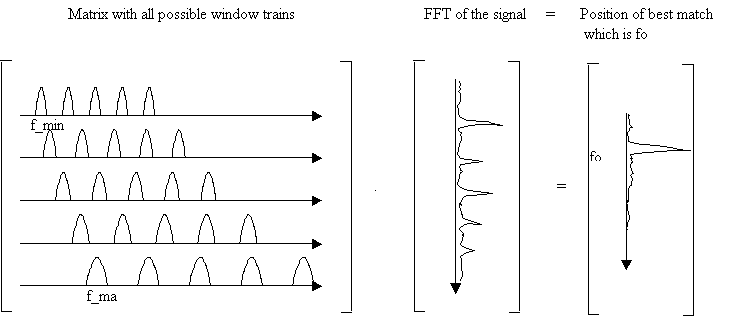
\includegraphics[scale=.4]{graph/pitch_maximumlikelihood}
		\end{figure}
        }
	\end{frame}
	
	\begin{frame}{fundamental frequency detection}{monophonic --- auditory-motivated pitch tracking 1/2}
		\begin{enumerate}
			\item	\textbf{filterbank} of band bass filters (e.g., mel scale)
			\pause
			\item	\textbf{HWR}
			\pause
			\item	\textbf{smoothing}
			\pause
			\item	within-band periodicity estimate (e.g. \textbf{ACF})
			\pause
			\item	\textbf{combination} of bands
		\end{enumerate}
	\end{frame}
	
	\begin{frame}{fundamental frequency detection}{monophonic --- auditory-motivated pitch tracking 2/2}
		\figwithmatlab{AuditoryPitchTracking}
	\end{frame}
	

   \section[summary]{lecture summary}
        \begin{frame}{summary}{lecture content}
            \begin{enumerate}
                \item   what are the basic properties of an audio signal that  $f_0$-detection algorithms take advantage of
                \smallskip
                \item<2->   name 3 time domain and 3 frequency domain approaches to $f_0$-detection algorithms
                \smallskip
                \item<3->   what are typical errors of the listed algorithms
                \smallskip
                \item<4->   describe how, for some $f_0$-detection algorithms, specific pre-processing options might improve the result
            \end{enumerate}
        \end{frame}
\end{document}

